%!TEX root = ../systemnahe-programmierung.tex

\chapter{Geschichte}\label{geschichte}

\begin{figure}[htbp]
\centering
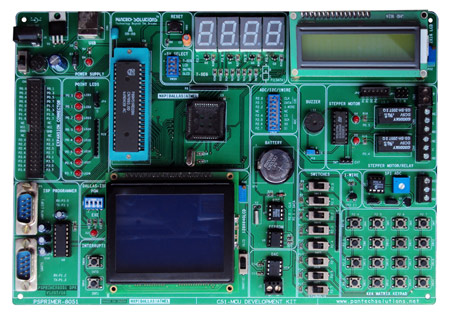
\includegraphics{images/8051-board}
\caption[8051 Board ]{8051 Board \footnotemark{}}
\end{figure}
\footnotetext{8051 Primer Board, https://www.flickr.com/photos/pantechsolutions/5760938387,
  Einsichtsnahme: 31.01.2015}

1980 präsentierte Intel den Nachfolger des 8048, den 8051. Er war als Erweiterung des 8048 zu sehen,
wurde von Intel intern als ``Verbesserte MCS-48 Architektur'' bezeichnent und enthielt somit
jegliche Funktionen dessen. Unteranderem wurden die Anzahl der Register mit 4 verdoppelt, ein
zweiter Timer eingeführt und diese auf 16-Bit aufgestockt.

Zum großen Erfolg des 8051 trug Intel mit den von Start ab vohandenen nötigen Programmen (Assembler,
Emulator, Software Beispielen) und der ausführlichen Dokumentation bei. So kamen bald verschiedene
Varianten ohne \ac{ROM} (8031) oder mit \ac{EPROM} (8751) auf und wurden bald durch noch bessere
Versionen mit mehr \ac{ROM}, \ac{RAM} und Timern ersetzt (z.B. 8052, 8kB \ac{ROM}, 256B \ac{RAM}, 3
16-Bit Timer). Durch die Lizensierung verschiedenster Firmen zur Herstellung des 8051 entstanden
immer mehr Varianten des ursprünglichen Microcontrollers. So z.B. in den 90ern Varianten mit Flash
Speicher um für Fehlerbehebungen oder neue Funktionen neu programmiert werden konnten und somit die
Kosten senkten.

Mit der großen Aktzeptanz des 8051 wurden die Applikationen immer größer und benötigten somit auch
mehr Leistung. Diese sollte eine 16-Bit Version des Controllers mit sich bringen, die kompatibel zur
ursprünglichen Version war. Nach dem Misserfolg dieser Variante konnten erst später Dritthersteller
eine erfolgreiche Variante mit mehr Megaherz auf den Markt bringen.